\chapter{Ergebnis} \label{Ergebnis}

Das Ziel bestand darin eine Grundstrucktur für ein GWT-Projekt zu erzeugen. 
Um das Projekt lauffähig zu machen, sind noch ein paar Handgriffe zu erledigen.
\begin{itemize}
  \item \textbf{Imports} \\
  Zum einen ist es notwendig die noch fehlenden Imports in den Java-Klassen
  einzufügen. 
  \item \textbf{AppEntryPoint.java} \\
  Hier muss defieniert werden welche der Views die Start Seite werden soll.
  \item \textbf{AbstractView.java} \\
  In dieser Klasse ist es möglich eine Standard Größe für die Seiten zu
  bestimmen.
  \item \textbf{ProductionGinModule.java} \\
  Auch hier muss wie in der AppEntryPoint-Klasse noch einmal die Start Seite
  definiert werden.
  \item \textbf{*.ui.xml} \\
  In diesen Dateien müssen doppelte Elemente entfernt werden, die der Generator zu
  viel eingefügt hat.
  \item \textbf{index.html und style.css} \\
  Diese beiden Dateien müssen nach dem durchlauf des Generators in den "`war"'
  Ordner kopiert werden. Sie dienen als Ausgangspunkt für die Webanwendung.
  \item \textbf{Zusätzliche Bibliotheken}\\
  	Zusätzlich zu den "`GWT SDK"' und "`App Engine SDK"' müssen die
    hier aufgeführten .jar Bibliotheken in das Projekt hinzugefügt werden.
  	\begin{itemize}
  	  \item \textbf{gin-2.0.jar}
  	  \item \textbf{guice-3.0-no\_aop.jar}
  	  \item \textbf{guice-assistedinject-3.0.jar}
  	  \item \textbf{gwt-servlet.jar}
  	  \item \textbf{javax.inject.jar}
	\end{itemize}
	
\end{itemize}

Sind diese Änderungen vorgenommen, ist das Projekt lauffähig. Nun können weitere
Änderungen vorgenommen werden, zum Beispiel können weitere Texte eingefügt
werden, natürlich kann auch das Design angepasst werden, dieses wurde von
Generator nur rudimentär, in Form einer einfaschen css-Datei angelegt.

\section{Beispiel Anwendung}
Für das in diesem Abschnitt gezeigte Beispiel wurde das Modell aus Abbildung
\ref{Fig:ergModell} verwendet. Zu sehen sind 5 Seiten, welche einzeln in
Paketen liegen, darüber hinaus wurden zwei PermanentViews modelliert, eine für
den Header, mit eingebautem Menu und eine für den Footer, in dem eine Navigation
zum Impressum vorgesehen ist.

\begin{figure}[htbp]
\begin{center}
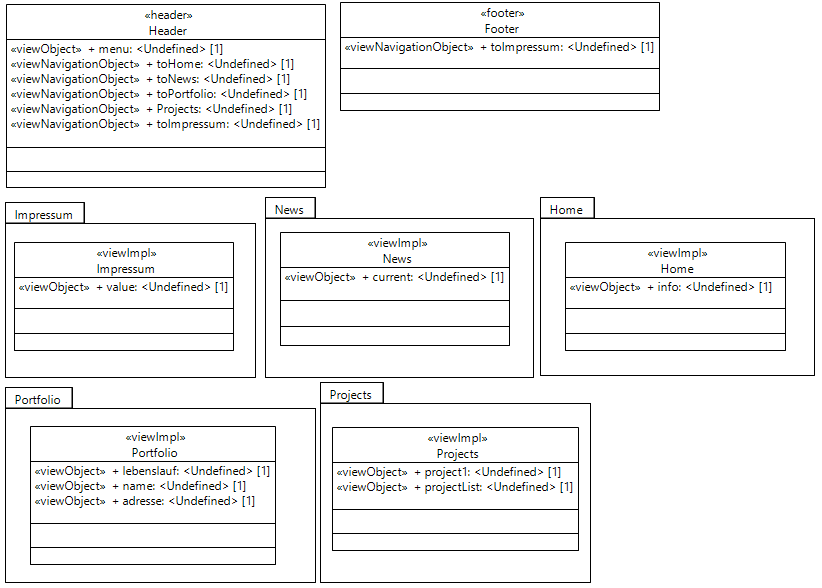
\includegraphics[width=0.8\textwidth]{./img/Model2.png}
\caption{Verwendetes Modell}\label{Fig:ergModell}
\end{center}
\end{figure}

Durch die extra eingebauten Pakete erweitert sich die Grundstrucktur des
Projektes, in Abbildung \ref{Fig:packegeModel} ist auf der linken Seite die
Komplette Packet-Struktur des Projektes zu sehen. Hier ist zu erkennen das es
für die fünf Seiten separate Pakete gibt, wobei für den Header und den Footer
keine zusätzlichen Pakete angelegt worden sind. Auf der rechten Seite der
Abbildung \ref{Fig:packegeModel}, wird der Inhalt einiger der Pakete näher
gezeigt, hier ist zu erkennen das die beiden \texttt{ViewImpl} die nicht in
Paketen liegen direkt in \texttt{view} Packet liegen, zusätzlich sind die erweiterten
Klassen \texttt{Activity}, \texttt{Place}, \texttt{View} und die
\texttt{.ui.xml} Datei in dem Packet zu sehen. Am Beispiel der "`Home"' Seite
ist gezeigt, dass die hierfür generierten Klassen und Dateien in einem separaten
unter Packet von \texttt{view}, nämlich \texttt{home} liegen.

\begin{figure}[htbp]
\begin{center}
\raisebox{3.2cm}{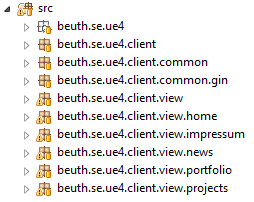
\includegraphics[width=0.4\textwidth]{./img/Packages.png}}
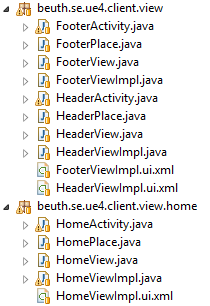
\includegraphics[width=0.4\textwidth]{./img/PackagesExample.png}
\caption{Generierte Paketstrucktur, links gesamte
Paketstrucktur im Überblick; rechts Beispiel für das
Strukturieren im Modell, mit zusätzlichen Paketen}\label{Fig:packegeModel}
\end{center}
\end{figure}
 
In diesem Beispiel soll die \texttt{home} Seite Den Start Punkt für die
Webanwendung darstellen, aus diesem Grund wurde entsprechend in der
\texttt{AppEntryPoint} und der \texttt{ProductionGinModule} die jeweilige Klasse
in für den Startpunkt angegeben. (Listing \ref{lst:appEntryPoint} und
\ref{lst:ProductionGinModule}) 
\lstset{language=gwt}
\begin{lstlisting}[caption={Änderung an der AppEntryPoint Klasse zur Bestimmung
der Startseite}, label={lst:appEntryPoint}] 
[..]
  historyHandler.register(injector.getPlaceController(), eventBus,
      new HomePlace());
[..]
\end{lstlisting}
\lstset{language=gwt}
\begin{lstlisting}[caption={Änderung an der ProductionGinModule Klasse zur Bestimmung
der Startseite}, label={lst:ProductionGinModule}] 
[..]
  bind(HomeView.class);
[..]
\end{lstlisting}

Zusätzlich wurde an einigen Stellen der Inhalt der Seiten erweitert, dies ist
einer seits dadurch möglich das innerhalb der \texttt{ViewImpl} Klasse zusätzlicher
Inhalt eingefügt werden kann, aber auch innerhalb der \texttt{.ui.xml} Datei,
beide verfahren werden hier anhand eines Beispiels gezeigt. Änderungen am
Java-Code siehe Listing \ref{lst:conntentJava} und innerhalb der UI-Datei siehe
Listing \ref{lst:conntentUI}.

\lstset{language=gwt}
\begin{lstlisting}[caption={Einfügen von Inhalten auf einer Seite durch
Veränderungen am Java-Code, hier in der \texttt{NewsViewImpl.java}},
label={lst:conntentJava}] 
[..] 
  HTML html = new HTML("<div><h1>Brandhei&szlig;e News</h1>"
	+"Lorem ipsum [..] amet."
	+"<div/>");
  content.add(html);
[..]
\end{lstlisting}
\lstset{language=gwt}
\begin{lstlisting}[caption={Einfügen von Inhalten auf einer Seite durch
Veränderungen am UI.XML-Datei, hier in der \texttt{HomeViewImpl.ui.xml}},
label={lst:conntentUI}] 
[..] 
 <g:FlowPanel>
	<!-- InteractionElements -->
	<!-- Start of user code Home 
	     Start protectetRegion -->
			<g:Label text=" Lorem [..] facilisi. "/>
			[..]		
	<!-- End of user code -->
	</g:FlowPanel>
[..]
\end{lstlisting}

Dies sind nur zwei Arten wie die Anwendung weiter bearbeitet werden kann,
nach dem der Quellecode aus dem M1-Model generiert worden ist. Zum einen
unterstützen der Generator und das Profil nicht alle, von GWT
bereitgestellten, UI-Elemente so, dass diese nachträglich eingefügt werden müssen.
Des Weiteren wurde sich in dieser Arbeit bewusst gegen das Erzeugen einer
Ausdesignten Webanwendung entschieden. Aus dem Grund, dass es diverse
Editoren gibt, welche das Erzeugen einer Benutzer Oberfläche graphisch
unterstützen.
